\chapter{Cinematica e dinamica relativistica}
\section{Cinematica relativistica}
\begin{definition}[Quadrivettore]
Consideriamo lo spazio vettoriale $\R^4$ con prodotto scalare indotto dal \textbf{tensore metrico di Minkovsky}
\[\eta_{\mu\nu}=\mat{1&&&\\
&-1&&\\
&&-1&\\
&&&-1}.\]
Un elemento di questo spazio \`e detto \textbf{quadrivettore}.
\end{definition}

\begin{definition}[Quadrivettore posizione]
Defniamo il \textbf{quadrivettore posizione} come
\[x^\mu=(ct,x,y,z).\]
In particolare $x^0=ct$, $x^1=x$, $x^2=y$ e $x^3=z$.\\
Come notazione scriviamo anche $\vec x=(x,y,z)$ e $\wt x=(ct,\vec x)$.
\end{definition}

\begin{notation}
Come notazione, se $\wt x$ \`e un quadrivettore posizione definiamo
\[s^2=\wt x\cdot \wt x=x^\mu\eta_{\mu\nu}x^\nu=(ct)^2-x^2-y^2-z^2.\]
\end{notation}

\begin{definition}[Quadrivettore di tipo tempo/spazio luce]
Affermiamo che un quadrivettore \`e di tipo 
\begin{itemize}
\item \textbf{tempo} se $s^2>0$
\item \textbf{spazio} se $s^2<0$
\item \textbf{luce} se $s^2=0$
\end{itemize}
Se il quadrivettore \`e di tipo tempo allora esso appartiene al \textbf{futuro} se $t>0$ o al \textbf{passato} se $t<0$.
\end{definition}

\begin{remark}
Un quadrivettore ortogonale ad uno di tipo tempo \`e di tipo spazio, ma un quadrivettore ortogonale ad uno di tipo spazio non necessariamente \`e di tipo tempo.
\end{remark}

\subsubsection{Causalit\`a}
\begin{proposition}[La causalit\`a viene rispettata]
Consideriamo due eventi $A$ e $B$. Se $\Delta t>0$ e $\Delta t'<0$ allora i due eventi non possono essere l'uno la causa dell'altro, cio\`e il quadrivettore dato dalla loro differenza \`e di tipo spazio.
\end{proposition}
\begin{proof}
Applicando la trasformazione di Lorenz
\[\Delta t'=\gamma\pa{\Delta t-\frac u{c^2}\Delta x}\]
dunque se $\Delta t'<0$ e $\Delta t>0$ allora
\[-\gamma\Delta t>-\gamma\frac u{c^2}\Delta x\implies \Delta x>\frac{c^2}{u}\Delta t>c\Delta t\]
cio\`e la distanza tra gli eventi \`e maggiore rispetto alla distanza che la luce potrebbe percorrere in quell'intervallo di tempo, quindi i due eventi non possono essere l'uno la causa dell'altro.
\end{proof}

\subsection{Derivazione delle trasformazioni di Lorenz}
Poich\'e le trasformazioni di Lorenz rappresentano un cambio di sistema di riferimento esse devono rispettare combinazioni lineari, cio\`e cerchiamo una trasformazione lineare.\\
Osserviamo che la norma di un quadrivettore posizione \`e esattamente l'intervallo invariante, quindi vogliamo che le trasformazioni siano isometrie per la metrica di Minkowski, cio\`e
\[\eta=L^\top\eta L.\]
\begin{remark}
Passando ai determinanti segue subito che $\det L=\pm 1$.
\end{remark}

\noindent Consideriamo l'equazione sopra in coordinate:
\[\sum_\nu\sum_\mu(L^\top)_{\al\mu}\eta_{\mu\nu}L_{\nu\beta}=\eta_{\al\beta}\]
nella convezione di Einstein possiamo evitare di scrivere i simboli di somma, dunque
\[\boxed{L_{\mu\al}\eta_{\mu\nu}L_{\nu\beta}=\eta_{\al\beta}}\]
Osserviamo che queste equazioni non cambiano scambiando $\al$ e $\beta$.\\
Come convenzione indici con lettere greche possono assumere valori tra $1$ e $4$, mentre indici latini solo tra $1$ e $3$.\\
Supponiamo che il moto avvenga lungo l'asse $x$ ($y'=y$, $z'=z$ e $x'$ non dipende da $y$ o $z$), cio\`e
\[L_{ij}=0 \quad \forall i,j\in\cpa{1,2,3},\ i\neq j\]
Consideriamo ora vari casi:
\begin{itemize}
\item Se $\al=i$ e $\beta=j$ per $i\neq j$ allora
\[L_{\mu i}\eta_{\mu\nu}L_{\nu j}=\eta_{ij}=0\implies L_{02}=L_{03}=0\]
\item Se $\al=0$ e $\beta=j$ allora
\[L_{\mu0}\eta_{\mu\nu}L_{\nu j}=\eta_{0j}=0\implies L_{00}L_{0j}-L_{j0}L_{jj}.\]
Intuitivamente $L_{00}$ e $L_{jj}$ non sono nulli perch\'e altrimenti $x'$ non dipenderebbe da $x$ e similmente per le altre componenti, quindi abbiamo trovato
\[L_{j0}=L_{0j}\frac{L_{00}}{L_{jj}}\]
In particolare $L_{20}=L_{30}=0$ e $L_{10}=L_{01}\frac{L_{00}}{L_{11}}$.
\item Se $\al=\beta=0$ allora abbiamo
\[L_{00}^2-L_{10}^2=\eta_{00}=1\]
\item Se $\al=\beta=i$ allora
\[L_{0i}^2-L_{ii}^2=\eta_{ii}=-1,\]
dunque $L_{01}^2=L_{11}^2-1$ e $L_{22}^2=L_{33}^2=1$.
\end{itemize}
\noindent
Battezziamo $L_{11}=\gamma>0$ e notiamo che
\[\begin{cases}
L_{10}=L_{01}\frac{L_{00}}{\gamma}\\
L_{01}=\pm\sqrt{\gamma^2-1}\\
L^2_{00}=L^2_{10}+1
\end{cases}\]
da cui
\[L_{00}^2=L_{00}^2\pa{1-\frac1{\gamma^2}}+1\implies L_{00}=\pm\gamma\]
e $L_{10}=\pm L_{01}=\pm \sqrt{\gamma^2-1}$.
\medskip

\noindent Mettendo tutto insieme (quindi anche $\det L=1$) troviamo la seguente forma per $L$\footnote{abbiamo supposto $L_{00}>0$ perch\'e altrimenti futuro e passato si scambierebbero}:
\[L=\mat{\gamma &\pm\sqrt{\gamma^2-1}&\\\pm\sqrt{\gamma^2-1}&\gamma&\\&&1&\\&&&1}\]
Queste sono esattamente le trasformazioni di Lorenz, infatti se $\gamma=\pa{1-\frac{u^2}{c^2}}^{-\frac12}$ allora $\sqrt{\gamma^2-1}=\frac uc\gamma$.



\subsection{Rapidit\`a}

\begin{definition}[Rapidit\`a]
Definiamo la \textbf{rapidit\`a} di un boost a velocit\`a $u$ come
\[\xi=\mathrm{arctanh}\pa{-\beta(u)}.\]
Segue che
\[\gamma(u)=\cosh\xi,\quad -\gamma(u)\beta(u)=\sinh\xi,\quad -\beta(u)=\mathrm{tanh}\, \xi.\]
\end{definition}
\begin{remark}
Si ha che
\[\mat{ct'\\ x'}=\mat{\cosh \xi &\sinh \xi\\\sinh \xi & \cosh \xi}\mat{ct\\ x},\]
cio\`e il boost corrisponde ad una rotazione iperbolica.
\end{remark}
\begin{remark}
L'identit\`a trigonometrica iperbolica
\[\cosh^2\xi-\sinh^2\xi=1\]
corrisponde a $\gamma^2(1-\beta^2)=1$, che \`e la definizione di $\gamma$.
\end{remark}


\begin{remark}
Considerando una composizione di velocit\`a 
\[u=\dfrac{u_1+u_2}{1+\frac{u_1u_2}{c^2}}\]
notiamo che le corrispondenti rapidit\`a si sommano\footnote{vedi le formule di prostaferesi per la tangente iperbolica (\ref{SommaTangenteIperbolica})}, cio\`e
\[\xi=\xi_1+\xi_2.\]
\end{remark}


\subsubsection{Diagramma di Minkowski}
Per semplicit\`a ignoriamo le componenti $y$ e $z$. Definiamo una base ortonormale dello spazio di Minkowski:
\[\wt e_0=\mat{\cosh \xi\\\sinh\xi},\quad \wt e_1=\pm \mat{\sinh \xi\\\cosh\xi}.\]
Poich\'e $\cosh^2\xi-\sinh^2\xi=1$, per ogni $\xi$ questi sono vettori di norma di Minkowski $1$, inoltre sono evidentemente ortogonali.
\bigskip

\noindent
Se $\wt e_0'$ e $\wt e_1'$ sono definiti come sopra ma a partire da una rapidit\`a $\xi'$ allora
\begin{align*}
\wt e_0\cdot \wt e_0'=&+\cosh(\xi-\xi')\\
\wt e_1\cdot \wt e_0'=&\pm \sinh(\xi-\xi')\\
\wt e_0\cdot \wt e_1'=&\mp\sinh(\xi-\xi')\\
\wt e_1\cdot \wt e_1'=&-\cosh(\xi-\xi')
\end{align*}

\noindent
Consideriamo ora un cambio di base
\[\wt a=x_0\wt e_0+x_1\wt e_1=x_0'\wt e_0'+x_1'\wt e_1'\]
Si pu\`o verificare che
\[\begin{cases}
\wt e_0=\cosh(\xi-\xi')\wt e_0'+\sinh(\xi-\xi')\wt e_1'\\
\wt e_1=\sinh(\xi-\xi')\wt e_0'+\cosh(\xi-\xi')\wt e_1'
\end{cases}\]
da cui ricaviamo
\[\begin{cases}
x_0'=x_0\cosh(\xi-\xi')+x_1\sinh(\xi-\xi')\\
x_1'=x_0\sinh(\xi-\xi')+x_1\cosh(\xi-\xi')
\end{cases}\]

\subsection{Tempo proprio e quadrivelocit\`a}
Poich\'e il tempo non \`e invariante per trasformazioni di Lorenz, non avrebbe senso definire una velocit\`a relativistica in termini solo del tempo. La generalizzazione giusta \`e la seguente

\begin{definition}[Tempo proprio]
Definiamo il \textbf{tempo proprio} come
\[\tau=\frac{\sqrt{s^2}}c.\]
Equivalentemente chiediamo che
\[d\tau^2=\frac{ds^2}{c^2}=dt^2-\frac1{c^2}\pa{dx^2+dy^2+dz^2}\]
\end{definition}

\begin{proposition}[Derivata del tempo rispetto al tempo proprio]\label{DerivataTempoPerTempoProprio}
Si ha che
\[\dd \tau t=\gamma(v),\]
dove $v=\sqrt{\pa{\dd tx}^2+\pa{\dd ty}^2+\pa{\dd tz}^2}$.
\end{proposition}
\begin{proof}
Sapendo che $d\tau^2=dt^2-\frac1{c^2}\pa{dx^2+dy^2+dz^2}$, ricaviamo che
\[d\tau^2=dt^2\pa{1-\frac{v^2}{c^2}}=\frac{dt^2}{\gamma(v)^2},\]
cio\`e
\[\dd \tau t=\gamma(v).\]
\end{proof}

\noindent Grazie al tempo proprio possiamo definire l'analogo relativistico della velocit\`a

\begin{definition}[Quadrivelocit\`a]
Definiamo la \textbf{quadrivelocit\`a} come
\[\wt v=\dd \tau{\wt x}=\dd \tau t\dd t{\wt x}=\gamma(v)\pa{c\dd tt,\dd t{\vec x}}=(c\gamma(v),\gamma(v)\vec v)=\gamma(v)(c,\vec v),\]
dove $\tau$ \`e il tempo proprio e $\vec v$ \`e la velocit\`a in senso non relativistico, cio\`e $\vec v=\dd t{\vec x}$.\\
La quantit\`a $\dd \tau{\vec x}=\gamma(v)\vec v$ \`e detta \textbf{velocit\`a propria}, \textbf{celerit\`a} o \textbf{velocit\`a relativistica}.
\end{definition}

\begin{remark}
La $4$-upla $(c,\vec v)$ NON \`e un quadrivettore perch\'e non \`e invariante cambiando sistema di riferimento, il fattore $\gamma(v)$ \`e dunque necessario per questo.
\end{remark}

\begin{remark}
Il modulo di Minkovski di una quadrivelocit\`a \`e
\[\wt v\cdot \wt v=c^2\gamma(v)^2-\vec v^2\gamma(v)^2=\gamma(v)^2(c^2-\vec v\cdot \vec v)=c^2\gamma(v)^2\pa{1-\frac{v^2}{c^2}}=c^2.\]
Segue in particolare che ogni quadrivelocit\`a \`e di tipo tempo.
\end{remark}

\noindent Se consideriamo un boost di velocit\`a $u$ parallela all'asse $x$ allora\footnote{$\gamma(u)$ e $\beta(u)$ non dipendono da $\tau$.}
\[\begin{cases}
\wt v_0'=\gamma(u)(\wt v_0-\beta(u)\wt v_1)\\
\wt v_1'=\gamma(u)(\wt v_1-\beta(u)\wt v_0)\\
\wt v_2'=\wt v_2\\
\wt v_3'=\wt v_3
\end{cases}\]

\begin{proposition}[Identit\`a tra i fattori $\gamma$]
Vale la seguente identit\`a
\[\gamma(v')=\gamma(u)\gamma(v)\pa{1+\frac{\vec u\cdot \vec v}{c^2}}\]
\end{proposition}
\begin{proof}
Osserviamo che
\[c\gamma(v')=\wt v_0'=\gamma(u)(\wt v_0-\beta(u)\wt v_1)=\gamma(u)(c\gamma(v)-\beta(u)\gamma(v)v_1),\]
dunque
\[\gamma(v')=\gamma(u)\gamma(v)\pa{1-\frac{v_1 u}{c^2}},\]
che \`e la tesi perch\'e supponiamo che $\vec u$ abbia la stessa direzione dell'asse $x$.
\end{proof}

\subsection{Quadriaccelerazione}
\begin{definition}[Quadriaccelerazione]
Definiamo la \textbf{quadriaccelerazione} come
\[\wt a=\dd\tau{\wt v}=\dd t{\wt v}\dd\tau t=\gamma(v)\dd t{}(c\gamma(v),\vec v\gamma(v))\]
\end{definition}
\begin{lemma}
Vale la seguente identit\`a
\[\boxed{\dd t{\gamma(v)}=\gamma(v)^3\frac{\vec v\cdot \vec a}{c^2}}\]
\end{lemma}
\begin{proof}
Calcoliamo:
\[\dd t\gamma=\dd t{}\pa{1-\frac{\vec v\cdot \vec v}{c^2}}^{-\frac12}=-\frac12\pa{1-\frac{\vec v\cdot \vec v}{c^2}}^{-\frac32}\pa{-\frac1{c^2}2\vec v\cdot \dd t{\vec v}}=\gamma(v)^3\frac{\vec v\cdot \vec a}{c^2},\]
in definitiva
\[{\dd t{\gamma(v)}=\gamma(v)^3\frac{\vec v\cdot \vec a}{c^2}}.\]
\end{proof}
\begin{corollary}
Segue dal lemma che
\[\dd t{}(\gamma(v)\vec v)=\gamma(v)^3\frac{\vec v\cdot \vec a}{c^2}\vec v+\gamma(v)\vec a.\]
\end{corollary}

\begin{remark}
Per quanto appena detto
\[\wt a=\pa{\gamma(v)^4\frac{\vec v\cdot \vec a}{c},\gamma(v)^4\frac{\vec v\cdot \vec a}{c^2}\vec v+\gamma(v)^2\vec a}=\gamma(v)^4\pa{\frac{\vec v\cdot \vec a}{c},\vec a+\frac{\vec v\times(\vec v\times \vec a)}{c^2}}\]
\end{remark}

\begin{remark}
Se $\vec a=0$ allora $\wt a=0$.
\end{remark}

\begin{remark}[Accelerazione propria]
Se ci troviamo un un sistema di riferimento a riposo ($\vec v=0$) allora $\gamma(v)=1$ e
\[\wt a=(0,\vec a).\]
In analogia a quanto detto possiamo definire $(0,\vec a)$ come l'\textbf{accelerazione propria}.
\end{remark}

\begin{remark}
Se l'accelerazione avviene lungo la direzione della velocit\`a allora
\[\wt a=\gamma(v)^4\abs{\vec a}(\beta(v),\wh v)\]
\end{remark}

\begin{remark}
Calcoliamo il seguente scalare, invariante per trasformazioni di Lorenz
\[\wt a\cdot \wt v=\dd[2]\tau{\wt x}\cdot \dd \tau{\wt x}=\frac12\dd\tau{}\pa{\dd \tau{\wt x}}^2=\frac 12\dd\tau{}(\wt v^2)=\frac 12\dd\tau c=0,\]
cio\`e la quadriaccelerazione e la quadrivelocit\`a sono sempre ortogonali per la metrica di Minkowski.
\end{remark}

\begin{remark}
Calcoliamo il modulo della quadrivelocit\`a
\[\wt a^2=\cdots=-\gamma(v)^4\vec a\cdot\vec a-\gamma(v)^6\frac{(\vec v\cdot \vec a)^2}{c^2}\]
in particolare $\wt a$ \`e un quadrivettore di tipo spazio.
\end{remark}

\begin{remark}
Supponiamo che $\vec v\perp \vec a$, allora
\[\wt a^2=-\gamma(v)^4\vec a\cdot \vec a,\]
che possiamo trovare dall'osservazione precedente o sfruttando l'equazione \[\wt a=\pa{\gamma(v)^4\frac{\vec v\cdot \vec a}{c},\gamma(v)^4\frac{\vec v\cdot \vec a}{c^2}\vec v+\gamma(v)^2\vec a}=(0,\gamma(v)^2\vec a)\]
\end{remark}




\section{Dinamica relativistica}
Cerchiamo di capire come leggere le leggi di Newton in chiave relativistica.\\
La prima legge \`e il primo postulato della relativit\`a ma con la seconda legge ($F=ma$) cominciamo ad avere qualche problema.\medskip

\noindent Per capire come procedere consideriamo il seguente esperimento

\begin{example}[Urto elastico di due palline identiche]
Fissiamo un sistema $S$ e cosideriamo un sistema $S'$ in moto relativo lungo l'asse $x$ a velocit\`a $u$. Due osservatori laciano delle palline ($1$ e $2$) lungo la direzione $y$ con la stessa velocit\`a in modo che queste si scontrino.\smallskip

\noindent Formalmente imponiamo
\[\begin{cases}
(v_1)_y=v_0\\
(v_1)_x=0\\
(v_2)_y'=-v_0\\
(v_2)_x'=0
\end{cases}\]
\begin{figure}[!htb]
    \centering
    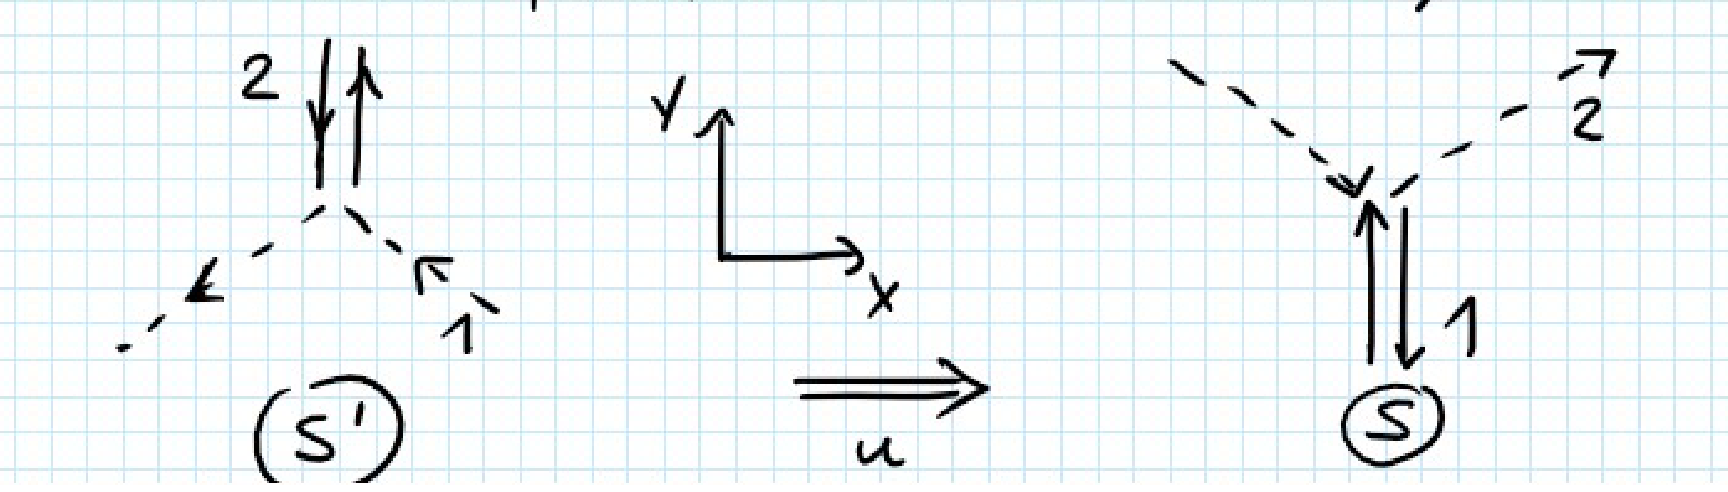
\includegraphics[width=9cm]{images/Palline_relativistiche_def_massa.png}
\end{figure}

\noindent
Considerando le formule di boost troviamo
\[\begin{cases}
(v_2)_x=\frac{0+u}{1+0}=u\\
(v_2)_y=\frac{-v_0}{\gamma(u)(1+0)}=-\frac{v_0}{\gamma(u)}.
\end{cases}\]
Imponiamo la conservazione degli impulsi (potenzialmente ammettendo che la massa dipenda dalla velocit\`a) lungo l'asse $y$:
\[2M(v_1)v_0=2M(v_2)\frac{v_0}{\gamma(u)},\]
da cui $\gamma(u)M(v_1)=M(v_2)$.\medskip

\noindent Ricordando\footnote{nota che $\vec u$ e $\vec v_1$ sono ortogonali} che $\gamma(v_2)=\gamma(v_1)\gamma(u)$ osserviamo che
\[\frac{M(v_2)}{\gamma(v_2)}=\frac{M(v_1)}{\gamma(v_1)}=\frac{M(0)}{\gamma(0)}=M(0)=m.\]

\end{example}

\begin{definition}[Massa a riposo]
Definiamo la \textbf{massa a riposo} $m$ come la massa misurata in un sistema dove il corpo \`e a riposo.
\end{definition}

\begin{definition}[Impulso relativistico]
Definiamo l'\textbf{impulso relativistico} come
\[\vec p=M(v)\vec v=m\gamma(v)\vec v.\]
\end{definition}
\begin{remark}
Con l'aumentare della velocit\`a, la ``massa effettiva" cresce molto fino a diventare ``infinita" per una velocit\`a che tende verso la velocit\`a della luce.
\end{remark}

\begin{definition}[Quadriimpulso]
Definiamo il \textbf{quadriimpulso} come
\[\wt p=m\wt v=(M(v)c,\vec p)=m\gamma(v)(c,\vec v).\]
L'impulso relativistico \`e la componente spaziale del quadriimpulso.
\end{definition}

\begin{remark}
Il modulo del quadriimpulso \`e
\[\wt p^2=m^2\wt v^2=m^2c^2.\]
In particolare il quadriimpulso \`e di tipo tempo (o di tipo luce se $m=0$).
\end{remark}

\noindent Abbiamo capito chi \`e la componente spaziale del quadriimpulso, ma la componente temporale?
\[\wt p_0c=m\gamma(v)c^2=m\gamma(v)c^2=\frac{mc^2}{\sqrt{1-\frac{v^2}{c^2}}}\]
per $v\to 0$ possiamo approssimare questa quantit\`a al primo ordine in $v^2$ come
\[mc^2-\under{\text{energia cinetica}}{\frac12 mv^2}\]

\begin{definition}[Energia]
Definiamo l'\textbf{energia} come $E=\wt p_0c$. In particolare se $v=0$ allora l'energia vale $mc^2$, che chiamiamo \textbf{energia di riposo}.
\end{definition}

\begin{remark}
L'esistenza dell'energia di riposo significa che se esiste un processo che fa diminuire la massa di un oggetto allora per conservazione dell'energia viene liberata dell'energia.\\
Questi processi esistono e vengono impiegati per l'estrazione di energia atomica.\\
Esistono processi che distruggono interamente la massa, per esempio lo scontro tra una particella e la sua antiparticella.
\end{remark}

\begin{remark}
Una volta definita l'energia possiamo riscrivere il quadriimpulso come
\[\wt p=m\wt v=(E/c,\vec p).\]
\end{remark}